% Desenvolvimento

\chapter{Desenvolvimento}

Este capitulo mostra as etapas de desenvolvimento da biblioteca e do jogo.

\section{Modelo de paraconsistente utilizado}

O modelo criado com a LPA foi implementado em uma dinâmica de ataque já adotada por jogos famosos como o \textit{Teamfight tactics} e o \textit{Dota Underlords}, se passando em um cenário onde todas as cartas devem atacar um único inimigo. Com a LPA é atribuído um benefício especial nessa dinâmica, possibilitando incluir valores contraditórios para os atributos das cartas, onde as regras de atribuição desses valores contraditórios podem vir por normas resultantes de mudanças de cenários, escolha de \textit{skills} e armamentos diferentes entre outras regras, por exemplo: Uma carta de um lutador de boxe que tem o atributo de força com o valor 88 e sua idade é de 60 anos, o valor contraditório sobre esse atributo pode ser mais que 70 pelo motivo de uma pessoa normal com mais de 60 anos possuir uma perda de massa muscular comum ao envelhecimento, além da diminuição de força nos membros inferiores

Foi criado um modelo para ser usado de base na criação da biblioteca que será usado para decidir o quanto as cartas atacando juntas conseguem tirar de vida de um adversário, criamos o modelo  com oito cartas e com os atributos de força, velocidade, cardio e experiência com valores favoráveis e desfavoráveis para os quatro atributos de cada carta conforme a tabela \ref{tab:cartas}.

\newpage

\begin{table}[htb]
	\centering
	\caption{Visualização das Cartas}
	\label{tab:cartas}
	\begin{tabular}{|l|l|l|l|}
		\hline
		\textbf{Carta}                        & \textbf{Atributos} & \textbf{Favoravel} & \textbf{Desfavoravel} \\ \hline
		\multirow{4}{*}{\textbf{Arqueiro}}    & velocidade         & 80                 & 67                    \\ \cline{2-4} 
		& força              & 20                 & 10                    \\ \cline{2-4} 
		& cardio             & 70                 & 68                    \\ \cline{2-4} 
		& experiência        & 60                 & 63                    \\ \hline
		\multirow{4}{*}{\textbf{Bárbaro}}     & velocidade         & 60                 & 63                    \\ \cline{2-4} 
		& força              & 75                 & 15                    \\ \cline{2-4} 
		& cardio             & 60                 & 65                    \\ \cline{2-4} 
		& experiência        & 40                 & 30                    \\ \hline
		\multirow{4}{*}{\textbf{Guerreiro}}   & velocidade         & 23                 & 60                    \\ \cline{2-4} 
		& força              & 80                 & 60                    \\ \cline{2-4} 
		& cardio             & 34                 & 70                    \\ \cline{2-4} 
		& experiência        & 30                 & 20                    \\ \hline
		\multirow{4}{*}{\textbf{Cavaleiro}}   & velocidade         & 68                 & 50                    \\ \cline{2-4} 
		& força              & 55                 & 40                    \\ \cline{2-4} 
		& cardio             & 64                 & 60                    \\ \cline{2-4} 
		& experiência        & 30                 & 69                    \\ \hline
		\multirow{4}{*}{\textbf{Espadachim}}  & velocidade         & 72                 & 50                    \\ \cline{2-4} 
		& força              & 56                 & 48                    \\ \cline{2-4} 
		& cardio             & 58                 & 5                     \\ \cline{2-4} 
		& experiência        & 59                 & 35                    \\ \hline
		\multirow{4}{*}{\textbf{Ancião}}      & velocidade         & 23                 & 68                    \\ \cline{2-4} 
		& força              & 44                 & 31                    \\ \cline{2-4} 
		& cardio             & 39                 & 68                    \\ \cline{2-4} 
		& experiência        & 77                 & 0                     \\ \hline
		\multirow{4}{*}{\textbf{Vikin}}       & velocidade         & 26                 & 50                    \\ \cline{2-4} 
		& força              & 45                 & 70                    \\ \cline{2-4} 
		& cardio             & 34                 & 80                    \\ \cline{2-4} 
		& experiência        & 77                 & 0                     \\ \hline
		\multirow{4}{*}{\textbf{Mosqueteiro}} & velocidade         & 53                 & 67                    \\ \cline{2-4} 
		& força              & 53                 & 10                    \\ \cline{2-4} 
		& cardio             & 53                 & 57                    \\ \cline{2-4} 
		& experiência        & 53                 & 52                    \\ \hline
	\end{tabular}
	\fonte{Produzido pelos autores.}
\end{table}

Esses detalhes das cartas e seus atributos podem ter uma ampla variedade, mudando de acordo com o tema do jogo de cartas.

No primeiro passo do modelo é realizado o processo de maximização, a partir do qual se obtém os maiores valores das evidências favoráveis e os menores das evidências desfavoráveis, levando em consideração o primeiro atributo de todas as cartas, realizando a maximização entre as cartas arqueiro e bárbaro, repetindo o processo em relação às cartas guerreiro e cavaleiro, espadachim e ancião, viking e mosquiteiro.

Depois é realizado o processo de maximização novamente com os valores resultantes da última maximização.

Na sequência, realiza-se o processo de minimização, no qual consiste na obtenção dos menores valores das evidências favoráveis e dos maiores valores das evidências desfavoráveis, as quais foram maximizadas anteriormente conforme a figura \ref{fig:oito}.

\begin{figure}[htb]
	\caption{
		\label{fig:oito}
		Extração da contradição entre as cartas
	}
	\begin{center}
		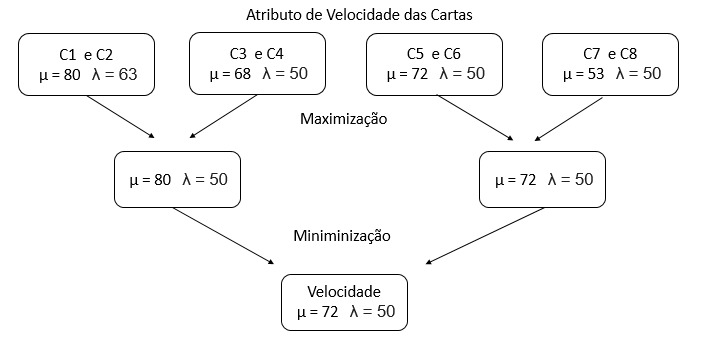
\includegraphics[scale=0.5]{imagens/valores.jpeg}
	\end{center}
	\legend{Fonte: Produzido pelos autores.}
\end{figure}	
	
Após realizar os processos de maximização e minimização o processo deve ser refeito com todos os atributos das cartas, resultando no seguinte resultado exibido na figura \ref{fig:atributo}:

\begin{figure}[htb]
	\caption{
		\label{fig:atributo} 
		Atributos
	}
	\begin{center}
		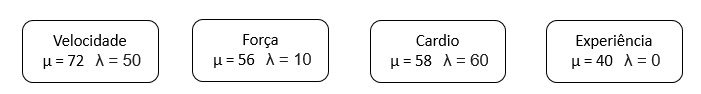
\includegraphics[scale=0.5]{imagens/atributo.jpeg}
	\end{center}
	\legend{Fonte: Produzido pelos autores.}
\end{figure}	

\newpage

Depois é realizado processo de maximização entre os atributos e depois minimização de acordo com a figura \ref{fig:valores_2}.

\begin{figure}[htb]
	\caption{
		\label{fig:valores_2} 
		Extração da contradição entre as cartas
	}
	\begin{center}
		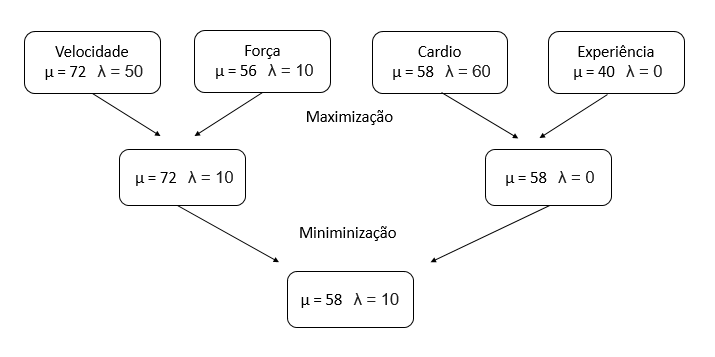
\includegraphics[scale=0.7]{imagens/valores_2.png}
	\end{center}
	\legend{Fonte: Produzido pelos autores.}
\end{figure}

Esses dois valores obtidos serão utilizados no algoritmo para-analisador. De maneira geral, para obter-se uma representação adequada da LPA e onde o resultado será inserido, utiliza-se um reticulado conforme a figura \ref{fig:reticulado}.	

\begin{figure}[htb]
	\caption{
		\label{fig:reticulado} 
		Reticulado
	}
	\begin{center}
		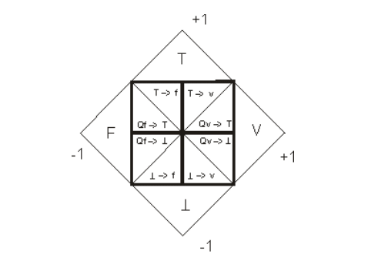
\includegraphics[scale=0.9]{imagens/reticulado.png}
	\end{center}
	\legend{Fonte: \citeauthor{tomda-decisao-lpa-2011}.}
\end{figure}

Como resultado das várias sentenças descritivas no reticulado representado no QUPC é proposto um algoritmo para implementação em um programa de computação convencional que possibilita a aplicação da LPA de anotação com dois valores LPA2v em Sistemas de Controle e Especialistas de IA, logo abaixo foi feito o algoritmo já com a implementação do modelo visto neste capítulo \cite{metodos-lpa-2006}.



\begin{figure}[htb]
	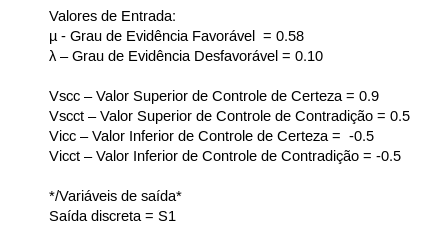
\includegraphics[scale=0.9]{imagens/codigo1.png}
\end{figure}

\begin{figure}[htb]
	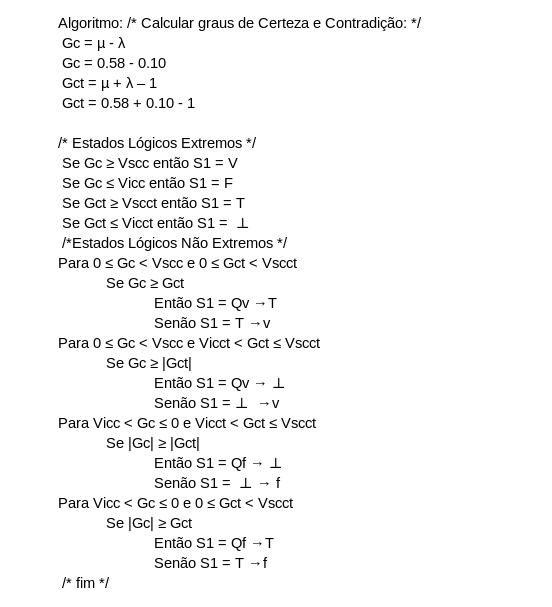
\includegraphics[scale=0.9]{imagens/codigo2.png}
\end{figure}

\newpage

Abaixo na tabela \ref{tab:estadosle} é demonstrado com tabelas a explicação de cada estado lógico.


\begin{table}[htb]
	\centering
	\caption{Estados lógicos extremos}
	\label{tab:estadosle}
	\begin{tabular}{ll}
		Estado 		& Definição     \\
		$V$     	& Verdadeiro    \\
		$F$     	& Falso         \\
		$\bot$     	& Indeterminado \\
		$T$     	& Inconsistente
	\end{tabular}
	\fonte{Produzido pelos autores.}
\end{table}

Além dos estados lógicos “extremos” a LPA2v permite a determinação de outros estados lógicos paraconsistentes listados abaixo conforme a tabela \ref{tab:estadosnle}:

\begin{table}[htb]
	\centering
	\caption{Estados lógicos não extremos}
	\label{tab:estadosnle}
	\begin{tabular}{|l|l|}
		\hline
		Estado & Definição                                  \\ \hline
		$T \rightarrow F$  		& Inconsistente tendendo ao falso            \\ \hline
		$T \rightarrow V$  		& Inconsistente tendendo ao verdadeiro       \\ \hline
		$\bot \rightarrow F$ 	& Indeterminado tendendo ao falso            \\ \hline
		$\bot \rightarrow V$    & Indeterminado tendendo ao verdadeiro       \\ \hline
		$Qf \rightarrow T$ 		& Quase falso tendendo ao inconsistente      \\ \hline
		$Qf \rightarrow \bot$   & Quase falso tendendo ao indeterminado      \\ \hline
		$Qv \rightarrow T$ 		& Quase verdadeiro tendendo ao inconsistente \\ \hline
		$Qv \rightarrow \bot$ 	& Quase verdadeiro tendendo ao indeterminado \\ \hline
	\end{tabular}
	\fonte{Produzido pelos autores.}
\end{table}

Aplicando o modelo criado no algoritmo paranalisador obtivemos o resultado: $\bot \rightarrow F$.

\newpage

O resultado lógico obtido foi indeterminado tendendo ao falso e através do estado lógico retornado foi produzido o parecer analítico com uma tabela \ref{tab:analitico}, cujo resultado refere-se a porcentagem que as oito cartas conseguem tirar de vida do adversário, nesse caso o ataque das oito cartas tirou 20\% da vida do adversário.


\begin{table}[htb]
	\centering
	\caption{Parecer analítico}
	\label{tab:analitico}
	\begin{tabular}{ll}
		Status             		& Parecer Analítico \\
		$V$                  	& 100\%               \\
		$Qv \rightarrow T$ 		& 90\%                \\
		$Qv \rightarrow \bot$ 	& 80\%                \\
		$T \rightarrow V$    	& 70\%                \\
		$\bot \rightarrow V$  	& 60\%                \\
		$T$                 	& 50\%                \\
		$\bot$                 	& 40\%                \\
		$T \rightarrow F$  		& 30\%                \\
		$\bot \rightarrow F$   	& 20\%                \\
		$F \rightarrow T$  		& 10\%                \\
		$F \rightarrow \bot$  	& 5\%                 \\
		F                    	& 0\%                
	\end{tabular}
	\fonte{Produzido pelos autores.}
\end{table}

O parecer analítico sobre os estados lógicos foi desenvolvido, com o pensamento de que quanto mais o resultado fosse verdade maior a porcentagem de vida que as cartas conseguem tirar do adversário.

Os resultados obtidos através do uso do algoritmo podem então ser utilizados em processos de tomada de decisão nas mais variadas áreas incluindo robótica e engenharia de controle \cite{aspectos-lpa-2013}.

\section{Criar da biblioteca para jogos de cartas}

Após a criação do modelo foi criado a primeira versão da biblioteca cuja sua  implementação foi feita na IDE Visual Studio criando uma projeto do tipo \textit{console application} ( aplicação console) devido sua facilidade e rapidez no desenvolvimento para realizar as validações e testes. Valendo do modelo conceitual já apresentado, a biblioteca foi criada seguindo a modelagem de classes UML na figura \ref{fig:classelpa} cujo detalhes estão no anexo do RUP.

\begin{figure}[htb]
	\caption{
		\label{fig:classelpa} 
		Diagrama de Classe
	}
	\begin{center}
		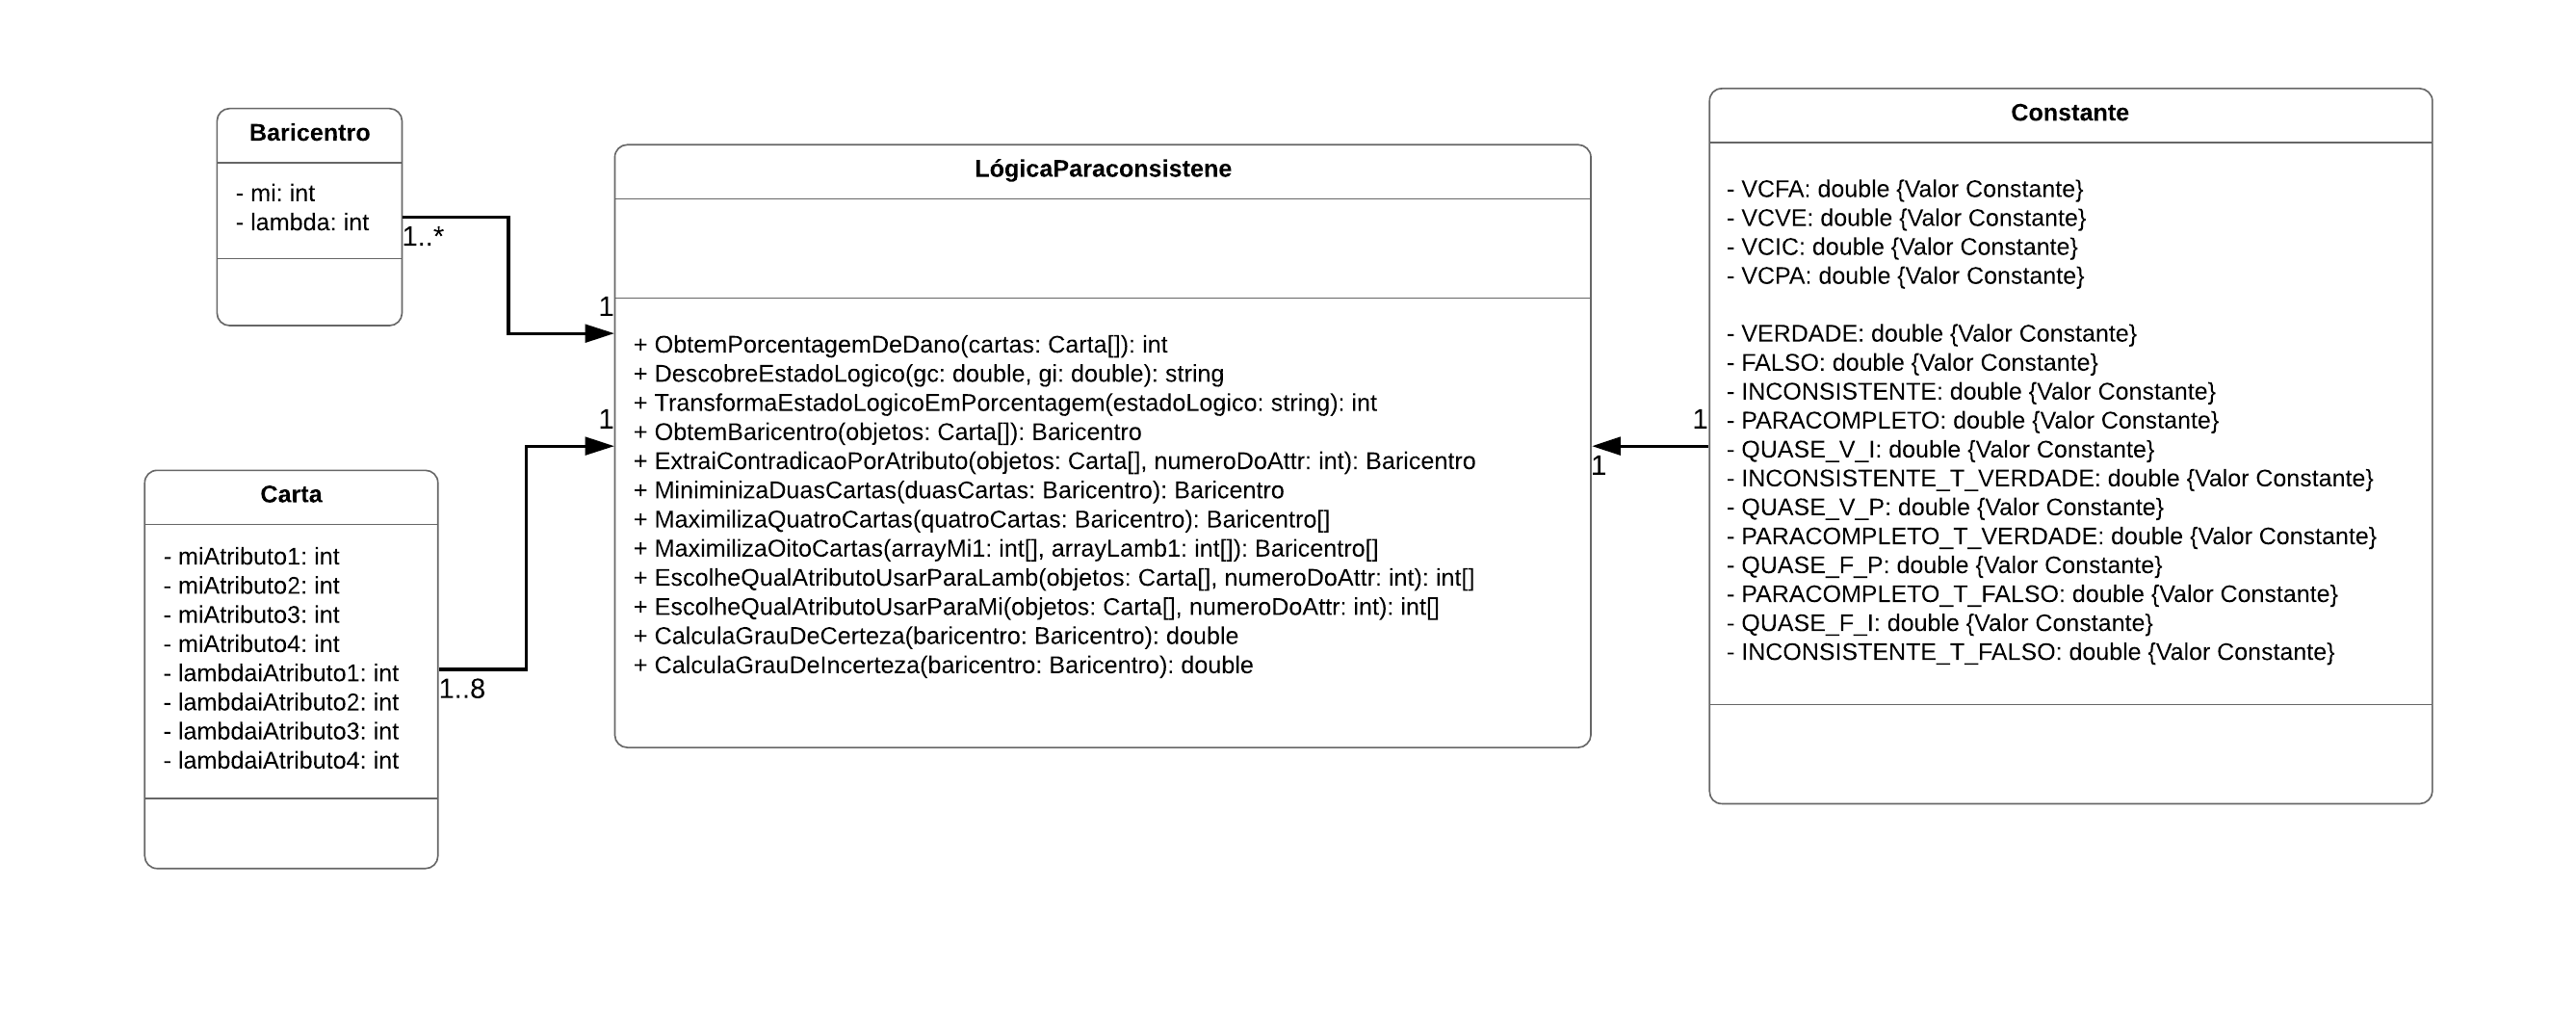
\includegraphics[scale=0.7]{imagens/classelpa.png}
	\end{center}
	\legend{Fonte: Produzido pelos autores.}
\end{figure}

\newpage

A primeira versão da biblioteca foi construída pensada em somente receber os parâmetros fixos das oito cartas com quatro atributos cada, assim a sua integração com o jogo seria mais rápida, e o protótipo do jogo já poderia ser desenvolvido.

Essa versão é composta de quatro classes, classe principal Lógica paraconsistente que é responsável pelo fluxo de extrair os valores da cartas, processar e apresentar na saída o valor em porcentagem do estado lógico resultante. As classes baricentro e carta são classes auxiliares para extração de valores, e a constante contém os valores fixo utilizada de parâmetro na lógica.

\section{Criação do jogo que integra a biblioteca}

O jogo foi desenvolvido com o intuito de provar a efetividade da biblioteca reunindo valores contraditórios retirando as contradições e tomando a decisão sobre o resultado da batalha.

O nome do jogo é \textit{Fighting Against Monsters}, o tema enquadrado se passa em diferentes cenários e as cartas são uma espécie de \textit{crossover} entre inúmeros personagens de quadrinho, desenhos animados e personagens criados pela equipe.

Com o jogo criado é possível demonstrar que a integração com a biblioteca é realizável. Em um primeiro momento o jogo contaria com oito cartas atacando um adversário. Foi alterado para entre as 8 cartas o jogador escolher quatro cartas para atacar assim adicionado uma maior jogabilidade, isso foi possível devido a segunda versão da biblioteca que será apresentado no próximo capítulo.

O método que foi chamado da biblioteca é o ObtemPorcentagemDeDano onde é passado como parâmetro um \textit{array} (Arranjo) de cartas e é retornado um inteiro com o número da porcentagem que as cartas que foram passadas como parâmetro conseguem tirar de vida do adversário. Esse método chama todos os outros métodos da biblioteca, extraindo a contradição e depois aplicando o algoritmo da paraconsistente, os outros métodos também podem ser chamados separadamente dependendo da aplicabilidade no jogo desenvolvido. Na figura \ref{fig:menu} está a tela inicial do jogo.

\begin{figure}[htb]
	\caption{
		\label{fig:menu} 
		Menu do Fighting Against Monsters
	}
	\begin{center}
		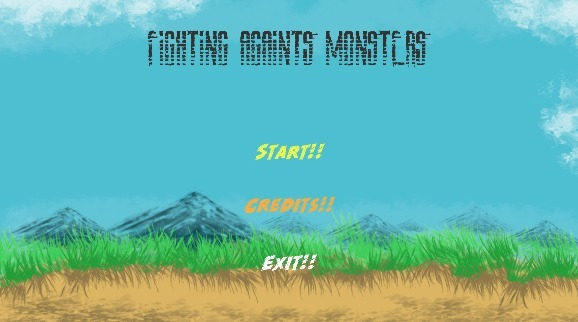
\includegraphics[scale=0.5]{imagens/menu.jpeg}
	\end{center}
	\legend{Fonte: Produzido pelos autores.}
\end{figure}

\newpage

Todas as cartas atacam o inimigo ao mesmo tempo e a lógica de ataque com o resultado é realizada pela biblioteca. Na figura \ref{fig:fase_1} e \ref{fig:fase_2} está a tela de combate.

\begin{figure}[htb]
	\caption{
		\label{fig:fase_1} 
		Tela de combate Fighting Against Monsters
	}
	\begin{center}
		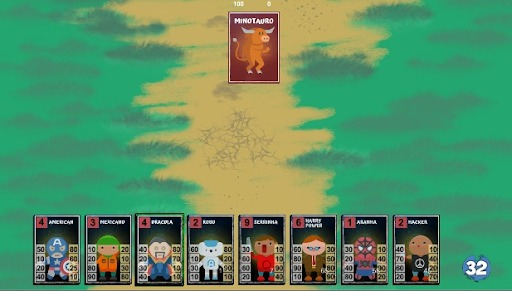
\includegraphics[scale=0.5]{imagens/fase_1.jpeg}
	\end{center}
	\legend{Fonte: Produzido pelos autores.}
\end{figure}

\begin{figure}[htb]
	\caption{
		\label{fig:fase_2} 
		Ataque das cartas
	}
	\begin{center}
		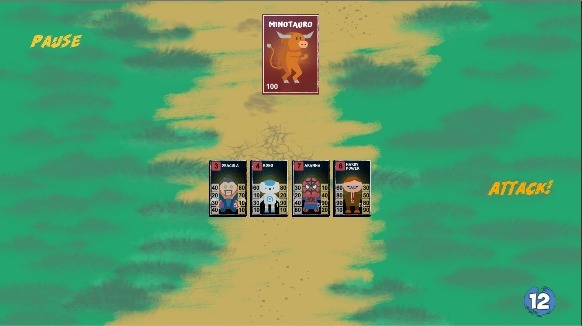
\includegraphics[scale=0.5]{imagens/fase_2.jpeg}
	\end{center}
	\legend{Fonte: Produzido pelos autores.}
\end{figure}


\section{Segunda versão da biblioteca}

Na segunda versão da biblioteca agora sendo nomeada com Decision Maker LPA, foi feito realizado uma refatoração na modelagem de classe, distribuindo a responsabilidade que antes estava exclusivamente na classe de lógica paraconsistente, adicionado melhor legibilidade ao código. Além disso, houve um aperfeiçoamento na implementação, possibilitando utilizar a biblioteca com quantidade de cartas da base dois.

O objetivo do desenvolvimento da biblioteca, além de expandir a LPA no mercado de jogos, é ajudar o desenvolvedor no unity a economizar horas em um projeto. Toda a construção da biblioteca foi mensurada em horas do início ao fim, no total foram 50 horas de desenvolvimento, ou seja, 50 horas que o desenvolvedor que baixar a biblioteca obterá de tempo economizado e conseguirá focar em outros pontos importantes, como nas regras de negócio do jogo. Essas horas foram mensuradas apenas para a biblioteca e não para o jogo, demonstrando que a biblioteca obteve maior tempo de desenvolvimento, devido ao fato de criação de design e script da lógica de jogos de cartas. 

\section{Disponibilização no Assets Store}

Como dito em capítulos anteriores o \textit{Unity} é a maior plataforma de desenvolvimento de jogos e a \textit{Unity Asset Store} é a plataforma para obter recursos pagos ou de graça para ajudar no desenvolvimento, esses recursos podem ser designs prontos, texturas, tutoriais, \textit{scripts}, ou jogos betas para serem usados de modelo no desenvolvimento.A \textit{Unity Asset Store} é uma biblioteca crescente de recursos, que são criados pela \textit{Unity Technologies} e pelos membros da comunidade e publicados na loja.

Por isso o \textit{Unity Assets Stores} é um dos lugares que a biblioteca e o jogo será disponibilizado

Em um primeiro momento foi pensado em cobrar pelo download do projeto, pois todos os recursos bons de design tem um preço razoável e os recursos de \textit{scripts} são geralmente bem mais caros, por estarmos disponibilizando os dois tipos de recursos, seria interessante cobrar por isso, porém a decisão da equipe foi não cobrar, pois para expandir a lógica paraconsistente no mercado de jogos a maneira mais rápida seria disponibilizar a biblioteca e o jogo de graça.